\documentclass{VUMIFPSbakalaurinis}
\usepackage{algorithmicx}
\usepackage{algorithm}
\usepackage{algpseudocode}
\usepackage{amsfonts}
\usepackage{amsmath}
\usepackage{bm}
\usepackage{caption}
\usepackage{color}
\usepackage{float}
\usepackage{graphicx}
\usepackage{listings}
\usepackage{subfig}
\usepackage{url}
\usepackage{wrapfig}
\usepackage[table,xcdraw]{xcolor}
\usepackage[backend=biber]{biblatex}
\usepackage{enumitem}\setlist{nosep}
\usepackage{listings}
\usepackage{color}

\definecolor{codegreen}{rgb}{0,0.6,0}
\definecolor{codegray}{rgb}{0.5,0.5,0.5}
\definecolor{codepurple}{rgb}{0.58,0,0.82}
\definecolor{backcolour}{rgb}{0.95,0.95,0.92}

\lstdefinestyle{mystyle}{
	backgroundcolor=\color{backcolour},   
	commentstyle=\color{codegreen},
	keywordstyle=\color{magenta},
	numberstyle=\tiny\color{codegray},
	stringstyle=\color{codepurple},
	basicstyle=\footnotesize,
	breakatwhitespace=false,         
	breaklines=true,                 
	captionpos=b,                    
	keepspaces=true,                 
	numbers=left,                    
	numbersep=5pt,                  
	showspaces=false,                
	showstringspaces=false,
	showtabs=false,                  
	tabsize=2
}

\lstset{style=mystyle}

% Titulinio aprašas
\university{Vilniaus universitetas}
\faculty{Informatikos Institutas}
\department{Programų sistemų katedra}
%\papertype{Bakalauro darbas}
\papertype{Bakalauro darbas}
\title{Anomalijų aptikimas interneto prieigos stebėsenos sistemos įrašuose}
\titleineng{Detection of anomalies in internet access monitoring system data}
\author{Jokūbas Rusakevičius}
\supervisor{asist. dr. Vytautas Valaitis}
\reviewer{j. asist. Linas Petkevičius}
\date{Vilnius – \the\year}

% Nustatymai
\setmainfont{Palemonas}  
\bibliography{bibliografija}

\begin{document}
\maketitle

\setcounter{page}{2}

\sectionnonumnocontent{Santrauka}
TODO: Santrauka
% Nurodomi iki 5 svarbiausių temos raktinių žodžių (terminų).
% Vienas terminas gali susidėti iš kelių žodžių.
\raktiniaizodziai{„MacroBase“, IPSS, analitinis įrankis, raktinis žodis 4, raktinis žodis 5}   

\sectionnonumnocontent{Summary}
TODO: summary
\keywords{„MacroBase“, IPSS, analitic engine, keyword 4, keyword 5}

\tableofcontents

\sectionnonum{Įvadas}
Šis darbas yra Programų Sistemų studijų baigiamasis bakalauro darbas apie anomalijų aptikimą interneto prieigos stebėsenos sistemos įrašuose naudojant „MacroBase“ atviro kodo analitinį įrankį bei „SQL“ paketą.

\subsectionnonum{Problematika}
Informacijos rinkimas fizine forma, juos užrašant ant popieriaus lapo, pasak MIT Media Lab direktoriaus Joi Ito, dar visai neseniai buvo vienintelis būdas rinkti, klasifikuoti ir saugoti duomenis. Žmogus mintis ir idėjas užrašydamas ant popieriaus lapo – paversdavo žiniomis (angl. \textit{knowledge}). Tačiau laikai keičiasi, ir dabartinė didžiųjų duomenų (angl. \textit{big data}) situacija yra kitokia. Dėl milžiniškų surenkamų duomenų kiekio, nėra trivialu atskirti naudingus ir nenaudingus duomenis, todėl, natūraliai, negalima visų surenkamų duomenų automatiškai priskirti prie ir vadinti žiniomis. Surinkti duomenys nėra žinios, kol jų nepradedama nagrinėti, analizuoti ir filtruoti, ir tik pradėjus šį procesą galima pastebėti, kad gaunama informacija yra įdomi ir netgi svarbi \cite{movie}.\par

Duomenų, kuriais yra operuojama, juos yra renkama ir saugoma, kiekiai nuolatos didėja \cite{iot}. Iš tiesų, dėl daugelio priežasčių net greitis, kuriuo šie duomenys yra generuojami eksponentiškai kyla \cite{zettabytes}. Jau 2015–2016 metais didžiosios socialinių tinklų kompanijos Twitter, Facebook ir LinkedIn pranešė fiksuojančios iki 12 milijonų įvykių (angl. \textit{events}) per sekundę \cite{twitter, facebook, linkedin}. Šie duomenų kiekiai gerokai lenkia žmogaus gebėjimą juos apdoroti bei žymiai apsunkina darbą tiek analitikams, tiek analitiniams įrankiams. Net aukščiausios kvalifikacijos (angl. \textit{best-of-class}) šių dienų taikomųjų programų operatoriai bei analitikai praneša panaudojantys anekdotiškai mažą jų surenkamų duomenų kiekį – mažiau nei 6\% \cite{prioritizing_attention}.\par

Renkant tokius didelius kiekius duomenų natūraliai, užfiksuojami įrašai, kurie yra nebūdingi įrašų rinkiniui bei išsiskiria. Duomenų vienetai nukrypę nuo kitų duomenų rinkinyje yra vadinami anomalijomis. Anomalijų aptikimas yra procesas, kurio metu yra aptinkama ir identifikuojama anomalija arba išskirtis (angl. \textit{outlier}) duomenų rinkinyje \cite{anomaly}. Šio darbo metu bus tiriamas anomalijų aptikimas remiantis belaidės interneto prieigos duomenų perdavimo spartos kontrolinių matavimų, atliktų 2014–2018 metais, rezultatais, kurie gauti naudojantis Lietuvos Respublikos ryšių reguliavimo tarnybos administruojama IPSS \cite{ipss}.\par

Fiksuojami esminiai ar sisteminiai duomenys tobulu atveju turėtų būti peržiūrimi reguliariai ir pilnai, tam kad būtų galima užtikrinti tolygią sistemų veiklą, matavimų taisyklingumą ar renkamų duomenų korektiškumą ir laiku identifikuoti bei eliminuoti kylančias klaidas bei užkirsti kelią kenkėjiškoms atakoms. Tačiau kaip jau minėta anksčiau, didėjantis duomenų kiekis gerokai lenkia žmogaus gebėjimą juos apdoroti. Duomenų kiekis nuolatos didėja, tačiau žmogaus dėmesys išlieką riboto dydžio. Iškyla iššūkis prioritetizuoti žmogaus dėmesį – akcentuoti, filtruoti, jungti, grupuoti ir kontekstualizuoti svarbiausius analizuojamų duomenų elgsenos ir būsenos pakitimus, taip padedant išskirti svarbiausius duomenų ypatumus ir rodyti žmogui tik apibendrintą, svarbia ir ribotą kiekį informacijos \cite{prioritizing_attention}. Visa nereikalinga informacija, kuri yra rodoma žmogui reikalauja ir eikvoja jo dėmesį \cite{attention}. Nors žmonėms yra fiziškai neįmanoma peržiūrėti visų duomenų, mašinos ir/ar kompiuteriai gali tai atlikti, ar bent gebėtų, jei jų resursai būtų ekonomiškai paskirstyti. Analitikų teigimu, didelis kiekis svarbių duomenų yra praleidžiama dėl neefektyvaus ir/ar lėto mašinų darbo \cite{prioritizing_attention}.\par

2017 metais Standfordo universitetas kartu su Masačusetso technologijos institutu paskelbė
kuriantys naują atviro kodo analitinį paieškos įrankį „MacroBase“. Šis įrankis yra skirtas ne tik darbui su didžiaisiais bet ir du greitaisiais duomenimis (angl. \textit{fast data}). Pagrindiniu uždaviniu „MacroBase“ sau išsikėlė žmogaus dėmesio prioritetizavimą. Vienas iš daugelio „MacroBase“ šio uždavinio sprendimų yra didžiausio dėmesio reikalaujančios išvesties sugeneravimas ir jos supaprastinimas, kur neįprastus duomenų vienetus „MacroBase“ padeda aiškinti pagal duomenų atributus \cite{macrobase_overview, prioritizing_attention, demonstration}. „MacroBase“ yra pakankamai naujas analitinis įrankis, gebantis grąžinti tikslius rezultatus dirbdamas 2 milijonų įvykių per sekundę, per užklausą, per branduolį greičiu, kuris taip pat pataikia daug inovatoriškų sprendimų vis didėjančių ir greitėjančių duomenų srautų analizei atlikti \cite{macrobase_overview}. Šiame darbe bus plačiau nagrinėjamas bei eksperimentai atliekami su „MacroBase“ įrankiu. Plačiau apie „MacroBase“ \ref{sec:macrobase} ir \ref{sec:macrobasesql} skyriuose.

\subsection{Darbo tikslai ir uždaviniai}
Šio darbo \textbf{tikslas} – ištirti „MacroBase“ duomenų analizavimo ir anomalijų aptikimo įrankio „SQL“ paketą – „MacroBase SQL“ ir pritaikyti jo veikimą analizavimui ir anomalijų aptikimui IPSS belaidės interneto prieigos duomenų perdavimo spartos kontrolinių matavimų įrašuose.\par

Darbui iškelti \textbf{uždaviniai}:
\begin{enumerate}
	\item Išanalizuoti „MacroBase SQL“ veikimo principą.
	\item Paruošti eksperimentinę aplinką ir IPSS įrašų rinkinį eksperimentui.
	\item Palyginti eksperimentų rezultatus, keičiant pagrindinių parametrų (procentilio, palaikymo ir rizikos koeficiento) reikšmes.
	\item Atlikti duomenų transformacijas (pridėti, atimti, filtruoti, keisti reikšmes) ir palyginti eksperimento rezultatus.
	\item Atlikti tas pačias transformacijas su kitais panašiais duomenimis ir palyginti eksperimento rezultatus. 
	\item Pateikti rekomendacijas IPSS duomenų anomalijų aptikimui naudojantis „MacroBase“.
\end{enumerate}

\section{„MacroBase“ analitinis įrankis} \label{sec:macrobase}
Šiame skyriuje yra aprašomas „MacroBase“ analitinis įrankis (\ref{subsec:about} poskyrius). Įranis kuriamas Standfordo Universiteto bedradarbiaujant kartu su Masačusetso technologijos institutu. Taip pat, šiame skyriuje rašoma apie „MacroBase“ žmogaus dėmesio prioritetizavimo bei kitų problemų sprendimo būdus (\ref{subsec:problems} poskyrius). 

\subsection{Apie „MacroBase“} \label{subsec:about}
„MacroBase“ nuo pradžių buvo kurtas būti žmogaus dėmesio prioritetizavimui skirtas analitinis įrankis, bet kad tai būtų pasiekta, reikia naudoti efektyvius aiškinamuosius ir klasifikavimo  statistinius operatorius, ir dirbti su duomenų srautais \cite{talk}. „MacroBase“ naudoja du pagrindinius operatorių tipus:
\begin{itemize}
	\item \textbf{Klasifikavimo} – tai operatorius, kuris pagal naudotojo nurodytas klases pats susižymi individualius taškus, kuriuos jau yra ištyręs (pavyzdžiui, statistiškai „normalus“ arba statistiškai „išskirtinis“).
	\item \textbf{Aiškinamieji} – tai operatoriai, kurie grupuoja ir jungia duomenų taškus po kelis.
\end{itemize}

Toliau trumpai aprašoma „MacroBase“ darbo proceso architektūra, kuri yra paremta dviem pagrindiniais principais. Pirma, visi operatoiai operuoja per duomenų srautus, jei duomenys yra išsaugoti ilgalaikėje atmintyje, prieš dirbant su šiais duomenimis, jie yra verčiami į srautus. Antra, „MacroBase“ yra paremtas kompiliatoriaus principu aprašytu žemiau, kuris užtikrina sąveiką tarp operatorių ir tvarkingą bendrą struktūrą \cite{macrobase_overview, kursinis}:
\begin{itemize}
	\item \textbf{Duomenų gavimas} (angl. \textit{ingestion}):
		\begin{itemize}
			\item „MacroBase“ gauna išorinį duomenų srautą analizei.
			\item Duomenų taškai susideda iš metrikų – matavimų (pavyzdžiui, greitism, kelionės laikas, baterijos procentai), ir atributų – siejamų duomenų (pavyzdžiui, telefono numeris, kompiuterio MAC adresas, paso kodas).
			\item „MacroBase“ anomalijų aptikimui naudoja metrikas, kurias po to paaiškina naudodama atributus.
		\end{itemize}
	\item \textbf{Duomenų transformavimas} (angl. \textit{feature transformation}):
		\begin{itemize}
			\item Tai yra neprivalomas procesas.
			\item Šio proceso metu „MacroBase“ vykdo domenui specifinių duomenų transformacijas. Šios transformacijos gali būti įvairių tipų: statistinės, priklausančios nuo duomenų tipo ar kt.
		\end{itemize}
	\item \textbf{Duomenų klasifikavimas} (angl. \textit{classification}):
		\begin{itemize}
			\item Kiekvienas duomenų taškas yra klasifikuojamas.
			\item „MacroBase“ šiuos taškus klasifikuoja jiems priskirdama po žymę, kuri yra priklausomą nuo metrikos.
			\item Taip pat, šioje proceso stadijoje yra treniruojamai klasifikatoriai. Klasifikatoriai yra treniruojami ir vertinami pagal srauto metrikas.
		\end{itemize}
	\item \textbf{Duomenų aiškinimas} (angl. \textit{explanation}):
		\begin{itemize}
			\item „MacroBase“ negrąžina tiesioginio sužymėtų duomenų taškų.
			\item „MacroBase“ sugeneruoja paaiškinimus ir apjungia sužymėto srauto duomenų taškus.
			\item Kadangi duomenų srauto duomenys yra nuolatos apdorojami, „MacroBase“ aiškinamieji operatoriai grąžina paaiškinimus tik gavusi naudotojo užklausą, taip išvengdamas nereikalingų skaičiavimų.
		\end{itemize}
	\item \textbf{Duomenų pateikimas} (angl. \textit{presentation}):
		\begin{itemize}
			\item Statistiniai reitingai yra priskiriami, dėl galimai didelio aiškinimų kiekio.
			\item „MacroBase“ naudotojams aiškinimus pateikia jų svarbos tvarka.
		\end{itemize}
\end{itemize}

\subsection{„MacroBase“ sprendžiamos problemos} \label{subsec:problems}
„MacroBase“ apibrėžia tris pagrindinius iššūkius, kuriuos turi įveikti greitųjų duomenų analizės sistemos. Šiame poskyriuje aprašomi šie dizaino iššūkiai ir kaip „MacroBase“ greito duomenų srauto analitinis įrankis juos sprendžia \cite{prioritizing_attention}:

Iškelti iššūkiai:
\begin{enumerate}
	\item Resursu nepakankamas kiekis jų interpretavimui.
	\item Resursu nepakankamas kiekis analizavimui.
	\item Resursų nepakankamas kiekis skaičiavimams.
\end{enumerate}

\subsubsection{Resursu nepakankamas kiekis jų interpretavimui}
Šio iššūkio įgyvendinimui „MacroBase“ naudoja jų vaidinamą – \textbf{išvesties prioritetizavimo principą}. Tai yra pasiekiama grąžinant daugiau informacijos su mažesne išvestimi. Kadangi kiekvienas duomenų vienetas reikalauja dėmesio, analitinis įrankis turi padaryti sprendimą, kokius duomenis rodyti naudotojui. Tai turi būti atlikta protingai ir pateikiami ne konkretūs, o apibendrinti ir sugrupuoti duomenų vienetai. \par

„MacroBase“ šis principas yra adaptuojamas leidžiant pasirinkti analizės metrikas ir atributus. Taip pat rodant anomalijas pasirinktai metrikai, kurias aiškina būtent pasirinkti atributai \cite{prioritizing_attention}.

\subsubsection{Resursu nepakankamas kiekis analizavimui}
Šio iššūkio įgyvendinimui „MacroBase“ naudoja jų vaidinamą – \textbf{iteracijų prioritetizavimo principą}. Analitinių sistemų vystymas turi būti paremtas iteracijomis ir grįžtamuoju ryšiu (anlg. \textit{feedback-driven}). Sistema turi suteikti naudingus numatytuosius nustatymus bei padaryti analitinio darbo procesą lengvai konfigūruojamą ir neversti naudotojų to daryti patiems. Pasikartojančios, klaidoms atsirasti aplinkybe suteikiančios ir varginančios užduotys turi būti automatizuojamos. Tuomet naudotojo darbas yra palengvinamas ir jo dėmesys sutelkiamas į taikomąją sričiai specifines žinias. \par

„MacroBase“ pateikia skirtingas skirtas įvairios kvalifikacijos analitikams ar panaudojimo sferoms. Papildomai, „MacroBase“ pateikia numatytuosius nustatymus, leidžiančius pradėti darbą tik įdiegus programinę įrangą ir juos redaguoti darbo proceso metu \cite{demonstration, prioritizing_attention}. Galiausiai, atviro kodo programinės įrangos „MacroBase“ internetiniame puslapyje galima užduoti klausimus ir pranešti apie sistemines klaidas.

\subsection{Resursų nepakankamas kiekis skaičiavimams}
Šio iššūkio įgyvendinimui „MacroBase“ naudoja jų vaidinamą – \textbf{skaičiavimų prioritetizavimo principą}. Analitinė sistema privalo prioritetizuoti skaičiavimus su duomenimis, darančius didžiausią įtaką rezultatui. Greičiausias būdas skaičiuoti (angl. \textit{compute}) – yra vengti skaičiavimų. Darbas su įvestimi turi būti prioritetizuojamas atsižvelgiant į išvestį, taip atliekant skaičiavimus su duomenimis, kurie prasideda labiausiai prie rezultato. Šioje vietoje yra labai naudingi inkrementiniai algoritmai, kurie ilgus ir daug resursų reikalaujančius skaičiavimus išsisaugo (angl. \textit{cache}) ir pakartotinai panaudoja. \par

„MacroBase“ analitinis įrankis prioritetizuoja skaičiavimus remdamasis galutiniais skaičiavimų rezultatais. Šiuo būdų ya  sutaupomas žymus kiekis nereikalingo darbo \cite{prioritizing_attention} ir „MacroBase“ gali pateikti skaičiavimų rezultatus greitai ir efektyviai.


\section{„MacroBase“ „SQL“ paketo veikimo principas – „MacroBase SQL“} \label{sec:macrobasesql}




\section{Duomenų analizės eksperimentas naudojant „MacroBase SQL“ modulį}
Eksperimentui atlikti buvo pasirinktas „MacroBase SQL“ analitinis įrankis „MacroBase“ su „SQL“ moduliu. Kadangi „MacroBase SQL“ yra leidžiama per komandinę eilutę, grafinė sąsajai kaip „MacroBase GUI“ naudota nebuvo. Atliekant eksperimentą buvo pasirinkti CSV tipo failų duomenų šaltiniai.

\subsection{Duomenų rinkinys}
Šiame skyriuje aprašyti eksperimentui pritaikyti duomenų rinkiniai.

\subsubsection{Eksperimentui pritaikyti duomenys}
Eksperimentui buvo naudojami Lietuvos Respublikos ryšių reguliavimo tarnybos administruojamos IPSS atliekami belaidės interneto prieigos duomenų perdavimo spartos kontrolinių matavimų 2014–2018 metų rezultatai. Matavimai atlikti operatorių UAB „Bitė Lietuva“, AB „Telia Lietuva“, UAB „TELE2“ ir AB LRTC judriojo ryšio tinkluose visoje Lietuvos teritorijoje. Matavimų paskirtis yra stebėti ir įvertinti teikiamų interneto prieigos paslaugų kokybę, kaip to reikalauja Europos Sąjungos direktyvos, taip pat supažindinti visuomenę su tokių matavimų rezultatais. Įrašai pateikiami CSV formato failais. Iš viso gauti 3 failai skirti trims skirtingoms technologijoms: 3G, LTE ir WiMAX. Viename CSV faile priklausomai nuo failui priskirtos technologijos buvo apytiksliai 136000, 157000 ir 18000 įrašų eilučių, vidutiniškai 104000. Vieno failo dydis vidutiniškai 8,5MB.

\subsubsubsection{Duomenų aprašymas}
Kiekvienas IPSS įrašų failas prasideda antraštės (angl. \textit{header}) eilute, kuri susideda iš faile saugomų įrašų sąrašo laukų (angl. \textit{fields}) pavadinimų. IPSS įrašų sarašų laukai ir jų paaiškinimas:

\begin{itemize}
	\item \textbf{Data ir laikas} – įrašo fiksavimo data ir laikas, užrašoma „yyyy-MM-dd hh:mm:ss“ formatu.
	\item \textbf{Platuma} – matavimo įrašo fiksavimo koordinačių platuma užrašoma dešimtainiais laipsniais (angl. \textit{decimal degrees}).
	\item \textbf{Ilguma} – matavimo įrašo fiksavimo koordinačių ilguma užrašoma dešimtainiais laipsniais (angl. \textit{decimal degrees}).
	\item \textbf{Operatorius} – matavimo įrašo operatoriaus skaitinis kodas arba pavadinimas (vieno iš jau minėtų operatorių: „Bitė Lietuva“, „Telia Lietuva“, „TELE2“ ar LRTC).
	\item \textbf{Ryšio tinklas} – tinklo technologija (3G, LTE arba WiMAX).
	\item \textbf{Celės id} – korinio tinklo ląstelės identifikacinis numeris atvaizduotas skaitine šešioliktaine forma.
	\item \textbf{Bazinės stoties id} – bazinės stoties identifikacinis numeris atvaizduotas skaitine šešioliktaine forma, parametras pateikiamas tik LRTC WiMAX tinkle atliktuose matavimuose.
	\item \textbf{3G ryšio technologija} – matavimų metu nustatytas duomenų perdavimo technologijos porūšis (WCDMA, HSPA+, DC-HSPA+).
	\item \textbf{RSSI} – (angl. \textit{Received Signal Strength Indicator}) signalo lygis, dBm (apklausiant modemą gaunamos vertės nuo -51 dBm iki -113 dBm. Mažiausia signalo vertė -113 dBm reiškia labai silpną signalą, kuriam esant praktiškai nebegalima naudotis duomenų perdavimo paslauga).
	\item \textbf{RSRP} – (angl. \textit{Reference Signal Received Power}) pilotinio signalo galia, dBm (apklausiant modemą gaunamos vertės nuo -140 dBm iki -44 dBm. Mažiausia signalo vertė -140 dBm reiškia labai silpną signalą, kuriam esant praktiškai nebegalima naudotis duomenų perdavimo paslauga). Parametras pateikiamas tik LTE tinkle atliktuose matavimuose.
	\item \textbf{RSRQ} – (angl. \textit{Reference Signal Received Quality}) pilotinio signalo kokybė, dB (apklausiant modemą gaunamos vertės nuo -19,5 dB iki -3 dB. Mažiausia vertė -19,5 dB). Parametras pateikiamas tik LTE tinkle atliktuose matavimuose.
	\item \textbf{SINR} – (angl. \textit{Signal to Interference and Noise Ratio})  signalo ir trukdžių plius triukšmo santykis, dB (apklausiant modemą gaunamos vertės nuo -20 dB iki 30 dB. Mažiausia vertė -20 dB). Parametras pateikiamas tik LTE tinkle atliktuose matavimuose.
	\item \textbf{CINR} – (angl. \textit{Carrier to Interference and Noise Ratio}) nešlio ir trukdžių plius triukšmo santykis, dB, parametras pateikiamas tik LRTC WiMAX tinkle atliktuose matavimuose.
	\item \textbf{Sparta kbit/s} – (angl. \textit{Download speed}) išmatuota duomenų gavimo spartos vertė, kbps.
\end{itemize}
IPSS matavimai atliekami naudojant Ryšių reguliavimo tarnybos turimą įrangą, kuri yra sumontuota matavimams skirtame automobilyje. Matavimai atliekami automobiliui judant (angl. \textit{drive test}) miestų gatvėmis, automagistralėmis arba rajoniniais keliais pagal pasirinktus maršrutus. Atliktų matavimų maršrutų bei koordinates galima pamatyti \ref{img:3G-0}, \ref{img:LTE-0} ir \ref{img:WiMAX-0} paveikslėliuose.
\begin{figure}[H]
	\centering
	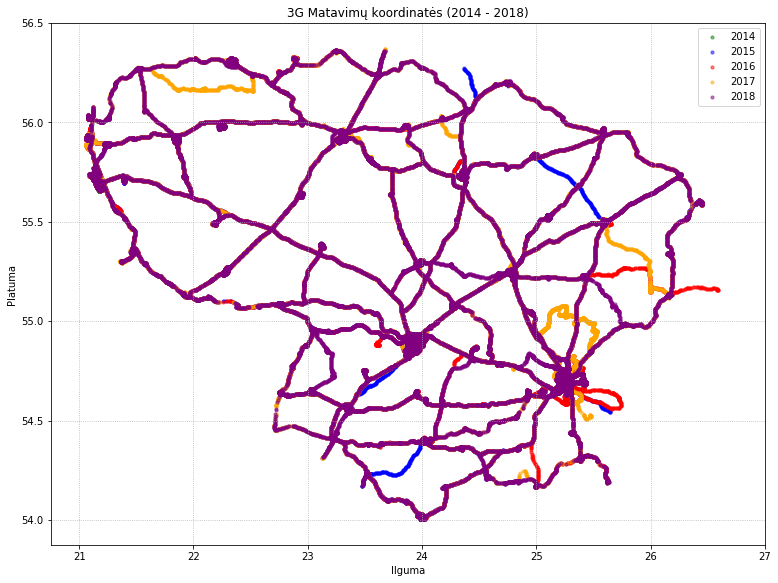
\includegraphics[scale=0.5]{img/3G-0}
	\caption{3G Matavimai 2014–2018 metais}
	\label{img:3G-0}
\end{figure}
\begin{figure}[H]
	\centering
	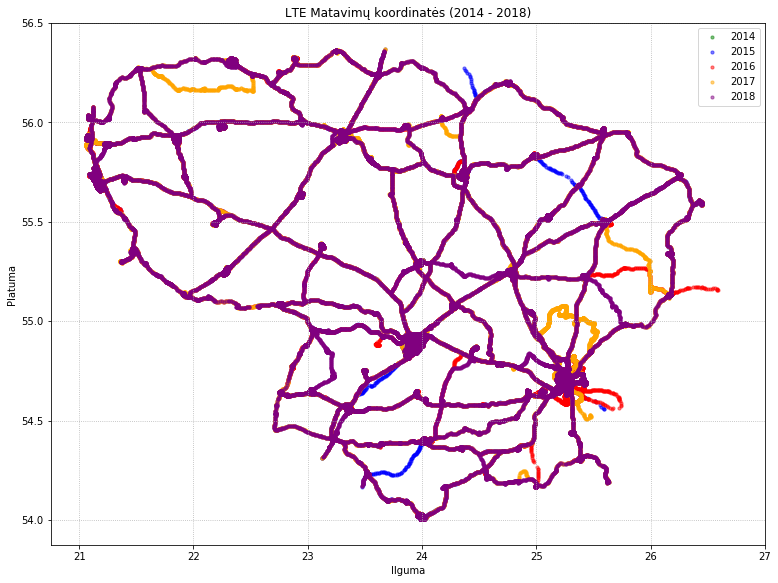
\includegraphics[scale=0.5]{img/LTE-0}
	\caption{LTE Matavimai 2014–2018 metais}
	\label{img:LTE-0}
\end{figure}
\begin{figure}[H]
	\centering
	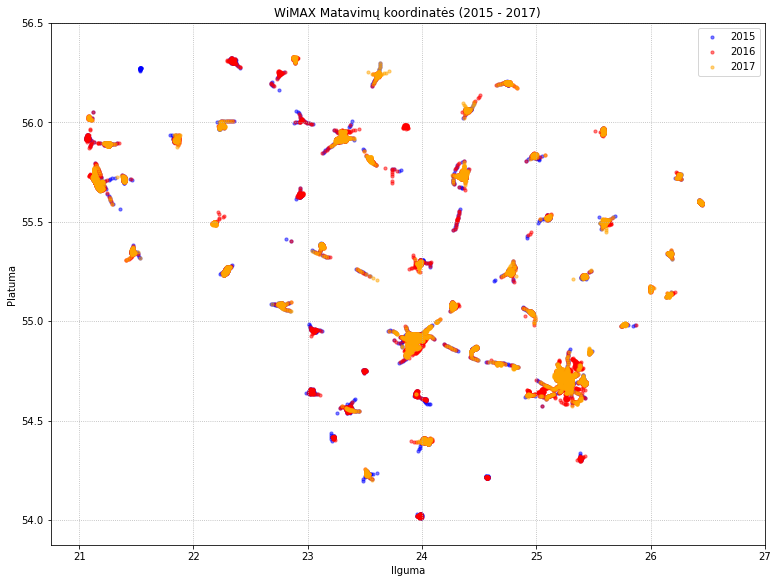
\includegraphics[scale=0.5]{img/WiMAX-0}
	\caption{WiMAX Matavimai 2015–2017 metais}
	\label{img:WiMAX-0}
\end{figure}
Aiškiau išskirtus įrašų koordinačių duomenis galima rasti Priede \ref{coordpav}.


\subsubsubsection{Pradinių duomenų paruošimas} \label{subsubsubsec:paruošimas1}
Eksperimentui atlikti buvo atrinkti laukai, kurie turi reikšmes visose įrašų sąrašo eilutėse bei taip pat buvo atmesti pasikartojančios informacijos laukai (ryšio tinklo ir ryšio technologijos laukai, kurie nurodo, koks tinklo tipas iš trijų tiriamųjų yra naudojamas faile). Taigi, 3G tinklui atrinkti šie pradiniai laukai: data, laikas, ilguma, platuma, operatorius, celės id, rssi, 3G ryšio technologija ir sparta; iš LTE duomenų atrinkti laukai: data, laikas, ilguma, platuma, operatorius, celės id, rssi, sparta; iš WiMAX duomenų atrinkti laukai: data, laikas, ilguma, platuma, operatorius, bazinės stoties id, rssi, sparta.\par

Eksperimentui atlikti buvo reikalingas CSV formato failai, kuriuose nebūtų lietuviškų raidžių ir būtų naudojami vieno žodžio arba vienos simbolių eilutės antraštės pavadinimai (pavyzdžiui, tarpai gali būti pakeičiami „\_“ simboliu), todėl buvo realizuotas „Python“ skriptas pavadintas „RenameAndRemoveFields.py“, kuris nuskaito duotųjų duomenų CSV failus ir juos apdorojus, grąžina naujus CSV failus. Skriptas, kaip ir visi darbo metu kurti skriptai, kurtas ir leistas „Jupyter Notebook“ aplinkoje. Skripte galima pasirinkti kelią iki duotųjų CSV failų ir kelią iki naujai sukuriamų CSV failų. Taip pat galima nurodyti norimas antraštes ir norimus laukus. Šio skripto paskirtis yra pervadinti antraštes ir atmesti nereikalingus laukus ir atskirti datą nuo laiko. Skriptas atlieka šiuos veiksmus 3 kartus kiekvienai ryšio technologijai (3G, LTE, WiMAX) (Priedas \ref{script1}):
\begin{enumerate}
	\item Nuskaito CSV įrašų failą pateiktą nurodytu keliu \textit{(18–23 ir 38 eilutės)}.
	\item Sukuria naują CSV failą nurodytų keliu ir pavadinimu \textit{(24 ir 39 eilutės)}.
	\item Sukuria „csv.writer“ objektą skirtą duomenų rašymui į CSV failus\textit{ (25 eilutė)}.
	\item Įrašo į naujai sukurtą CSV failą, naują antraštę, su naujais angliškais vieno žodžio (simbolių eilutės) pavadinimais \textit{(26 eilutė)}.
	\item Vykdo ciklą, kuris iš pradinio failo nuskaitytų duomenų kiekvieno įrašo atrenka reikalingus laukus, atskiria laiką nuo datos ir įrašo į CSV failą naujai sukurtą eilutę. Taip pat atlieką kiekvienos eilutės skaičiavimą \textit{(28–34 eilutės)}.
	\item Išvedamas galutinis eilučių skaičius \textit{(35 eilutė)}.
	\item Į konsolę išvedama operacijos užbaigimo žinutė \textit{(40 eilutė)}.
\end{enumerate}

\subsubsubsection{Papildytų duomenų paruošimas: koordinačių suapvalinimas, aukščio virš jūros lygio pridėjimas} \label{subsubsubsec:paruošimas2}
IPSS duomenyse yra pateikta daug informacijos, tačiau, dėl didelės jų įvairovės ir dėl realių skaičių laukuose, tik maža dalis jų yra potencialiai panaudojama aiškinimo procesui. Todėl buvo sukurtas antras skriptas pradinių duomenų papildymui  (papunktis \ref{subsubsubsec:paruošimas1}). Skripto paskirtis buvo pridėti papildomus koordinačių laukus, kuriuose būtų tos pačios koordinatės tačiau suapvalintos iki pasirinkto skaičiaus po kablelio. Skriptas turėjo ir antrą uždavinį – pasinaudojus tiksliomis, originaliomis koordinatėmis rasti aukštį virš jūros lygio ir pridėti šią bei suapvalintą reikšmes į joms skirtus naujus laukelius. Šis skriptas buvo pavadintas „AddAltitudeAndRoundedColumns.py“. Skriptas leidžia pasirinkti kelią iki pradinio CSV failo, kelią iki naujai sukuriamo CSV failo, taip pat skaitmenų po kablelio apvalinimo skaičių, bei aukščio virš jūros lygio apvalinimo sąlygas. Kadangi skriptas naudoja „Jawg.io“ API, jam reikia pateikti vartotojo prieigos žymę (angl. \textit{access token}). Taigi naujas „Python“ skriptas nuskaito prieš tai sukurtus CSV failus, gauna aukščio virš jūros lygio reikšmes, suapvalina koordinačių bei aukščio reikšmes ir sukuria naujus CSV failus pasirinktu keliu ir pavadinimu. Skriptas atlieka šiuos veiksmus 3 kartus kiekvienai ryšio technologijai (3G, LTE, WiMAX) (Priedas \ref{script2}):
\begin{enumerate}
	\item Nuskaito CSV įrašų failą pateiktą nurodytu keliu bei atskiria antraštę nuo įrašų \textit{(9–13 ir 89 eilutės)}.
	\item Iš antraštės surandami platumos ir ilgumos laukų indeksai \textit{(14–17 ir 90 eilutės)}.
	\item Pasinaudojus gautais indeksais, sukuriami visų ilgumos ir platumos reikšmių masyvai \textit{(18–21 ir 91 eilutės)}.
	\item Kadangi bus atliekamos HTTP užklausos ir URL užklausos ilgis yra ribots, yra vykdomas ciklas, kuris visus įrašus padalina į pasirinkto žingsnio dydžio dalis \textit{(22–34 ir 92)}.
	\item Vykdomas ciklas cikle, kuris visas ilgumos ir platumos reikšmes sujungia į „string“ tipo kintamuosius, kuriuose ilguma ir platuma yra atskirtos kableliu „,“\textit{ (26–31 eilutės)}.
	\item Kiekvienam žingsniui, iš platumos ir ilgumos bendrų kintamųjų sukuriamas vienas „string“ kintamasis, kur kiekvienas koordinačių poros kintamasis yra atskirtas vertikaliu brūkšniu „|“ \textit{(33 eilutė)}.
	\item Vykdomas ciklas, kuris kiekvienai žingsnio koordinačių kiekio „string“ kintamajam sukuria URL užklausą „Jawg.io“ API, kuri susideda iš koordinačių kintamojo, pagrindinio URL ir vartotojo prieigos žymės (angl. \textit{access token}) \textit{(35–40 ir 93 eilutės)}.
	\item Kiekvienam žingsniui yra siunčiama HTTP užklausa, kuri grąžina JSON duomenų struktūrą su koordinatėmis ir jų aukščiais virš jūros lygio \textit{(41–44 eilutės)}.
	\item Iš JSON duomenų struktūros atskiriamos aukščio virš jūros lygio reikšmės ir jos yra patalpinamos į masyvą atitinkamu indeksu \textit{(45 eilutė)}.
	\item Kas 100 žingsnių yra atspausdinamas atliktų žingsnių kiekis (naudotas žingsnio dydis – 100 įrašų, todėl spausdinama, kas 10000 įrašų), tai atliekama, kad būtų galima stebėti procesą, ypač, kadangi tinkle atliekamos operacijos yra lėtesnės ir yra ribotas „Jawg.io“ API duodamų operacijų skaičius \textit{(37 ir 47–49 eilutės)}.
	\item Vykdomas ciklas, kuris kiekvienam nuskaitytam įrašui sukuria nauja įrašą su suapvalintomis iki pasirinkto skaičiaus po kablelio reikšmėmis bei aukščio virš jūros lygio ir suapvalinta iki dešimčių aukščio virš jūros lygio reikšmėmis. Šie įrašai sujungiami su atitinkamais įrašais ir sukuriamas naujas sąrašas su šiais įrašais \textit{(51–65 ir 94 eilutės)}.
	\item Sukuriami nauji laukų antraštės pavadinimai bei pertvarkomos naujai pridėtų laukų (suapvalintų ir aukščio reikšmių) pozicijos \textit{(47–87 ir 95 eilutės)}.
	\item Sukuriamas naujas CSV failas nurodytu keliu ir pavadinimu \textit{(66–72 ir 96 eilutės)}.
	\item Įrašoma nauja antraštė su papildytais pavadinimais \textit{(69 eilutė)}.
	\item Vykdomas ciklas, kuris kiekvieną naujo įrašų sąrašo elementą įveda į jam skirtą naujo CSV failo poziciją \textit{(70–72 eilutės)}.
	\item Išvedama operacijos užbaigimo žinutė \textit{(97 eilutė)}.
\end{enumerate}

\subsubsubsection{Papildytų duomenų paruošimas: metų ir valandų išskyrimas} \label{subsubsubsec:paruošimas3}
Ruošiant IPSS duomenis eksperimentui jau buvo panaudota didžioji dalis originaliai paruoštų duomenų laukų (papunkčiai \ref{subsubsubsec:paruošimas1} ir \ref{subsubsubsec:paruošimas2}). Tačiau dėl didesnio potencialių aiškinamųjų laukų kiekio buvo sukurtas skriptas išskirti valandas iš laiko lauko (pvz. iš „09:15:39“ gaunama „09“), kadangi laiko laukas buvo nenaudojamas ir metus iš datos lauko (pvz. iš „2015-09-13“ gaunama „2015“). „Python“ skriptas pavadintas „AddYearAndHour.py“. Naudojantis skriptu, galima nurodyti pradinių CSV failų kelius ir naujų CSV failų kelius. Skriptas atlieka šiuos veiksmus 3 kartus kiekvienai ryšio technologijai (3G, LTE, WiMAX) (Priedas \ref{script3}):
\begin{enumerate}
	\item Nuskaito CSV įrašų failą pateiktą nurodytu keliu bei atskiria antraštę nuo įrašų \textit{(6–10 ir 39 eilutės)}. 
	\item Iš antraštės surandami datos ir laiko laukų indeksai \textit{(11–14 ir 40 eilutės)}.
	\item Vykdomas ciklas, kuris kiekvienam nuskaitytam įrašui sukuria nauja įrašą į kurį yra įterpiamos naujos metų ir valandų reikšmės į joms skirtas vietas. Šie įrašai sujungiami ir sukuriamas naujas sąrašas \textit{(15–24 ir 41 eilutės)}.
	\item Sukuriami nauji laukų antraštės pavadinimai su įterptomis naujomis metų ir valandų reikšmėmis, joms skirtose pozicijose \textit{(25–31 ir 42 eilutės)}.
	\item Sukuriamas naujas CSV failas nurodytu keliu ir pavadinimu \textit{(32–37 ir 43 eilutės)}.
	\item Įrašoma nauja antraštė su papildytais pavadinimais \textit{(34 eilutė)}.
	\item Vykdomas ciklas, kuris kiekvieną naujo įrašų sąrašo elementą įveda į naują CSV failą \textit{(36–37 eilutės)}.
	\item Išvedama operacijos užbaigimo žinutė \textit{(44 eilutė)}.
\end{enumerate}

\subsubsubsection{Papildytų duomenų paruošimas: apvalinimo variacijos} \label{subsubsubsec:paruošimas4}
Eksperimentui atlikti jau buvo sukurta pakankamai laukų (papunkčiai \ref{subsubsubsec:paruošimas1}, \ref{subsubsubsec:paruošimas2} ir \ref{subsubsubsec:paruošimas3}), tačiau patikrinti, kuri apvalinimo aukščio ir koordinačių kombinacija yra geriausia ir paaiškina daugiausiai anomalijų, reikia sugeneruoti daugiau duomenų rinkinių. Tam buvo parašytas dar vienas „Python“ skriptas – „GenerateMoreRoundedOptions.py“. Šis skriptas leidžia pasirinkti pradinius CSV failus, norimus testuoti intervalus koordinačių apvalinimui ir aukščio virš jūros lygio apvalinimui. Šiems intervalams yra sugeneruojamas po įrašų rinkinys, kurie yra išsaugomi pasirinktu pavadinimu ir keliu. Koordinačių apvalinimas vyksta skaitmenų po kablelio kiekio keitimu \textit{[0, inf)}, aukščio virš jūros lygio apvalinimas vyksta iki dešimčių dalių \textit{(0, inf)} (pvz. dalinama į 1 dalį ir apvalinama iki – „10 20 30...“; į 2 dalis – „5 10 15...“; 3 – „3,33 6,67 10...“ ir t.t.). Taigi, šis skriptas pagal duotą pradinį duomenų rinkinį generuoja kiekvienam intervalų atvejui po naują duomenų rinkinį. Skriptas atlieka šiuos veiksmus 3 kartus kiekvienai ryšio technologijai (3G, LTE, WiMAX) (Priedas \ref{script4}):
\begin{enumerate}
	\item Nuskaito CSV įrašų failą pateiktą nurodytu keliu bei atskiria antraštę nuo įrašų \textit{(6–10 ir 34 eilutės)}. 
	\item Iš antraštės surandami ilgumos, platumos, aukščio virš jūros lygio bei jų suapvalintų reikšmių laukų indeksai \textit{(11–18 ir 35 eilutės)}.
	\item Vykdomas ciklas cikle, kuris kiekvienai apvalinimo iki skaitmenų po kablelio ir kiekvienai aukščio virš jūros lygio apvalinimo parinkčiai sugeneruoja po atskirą failą \textit{(36–43 eilutės)}.
	\item Kiekvienam failui sukuriamas naujas unikalus pavadinimas \textit{(25–26 ir 36 eilutės)}.
	\item Vykdomas ciklas, kuris platumo, ilgumos ir aukščio reikšmes suapvalinta iki nurodytos reikšmės ir pakeičia senas suapvalintas reikšmes naujomis. \textit{(19–24 ir 39 eilutės)}.
	\item Sukuriamas naujas CSV failas nurodytu keliu ir pavadinimu \textit{(27–32 ir 40 eilutės)}.
	\item Įrašoma nauja antraštė su papildytais pavadinimais \textit{(30 eilutė)}.
	\item Vykdomas ciklas, kuris kiekvieną atnaujinto įrašų sąrašo elementą įveda į naują CSV failą \textit{(31–32 eilutės)}.
	\item Išvedama vienos operacijos užbaigimo žinutė \textit{(40 eilutė)}.
	\item Išvedama ciklo užbaigimo žinutė \textit{(41 eilutė)}.
	\item Išvedama visų operacijų užbaigimo žinutė \textit{(42 eilutė)}.
\end{enumerate}
 
Eksperimentui atlikti buvo nuskaityti ir apdoroti apie 300000 įrašų, vidutiniškai 100000 per failą.
TODO: pridėti citatą
\subsection{Eksperimento aplinkos paruošimas}
Eksperimentas buvo atliekamas naudojant „Ubuntu (64-bit)“ operacinę sistemą įdiegtą virtualioje mašinoje „Oracle VM VirtualBox“. „MacroBase SQL“ įdiegtas ir paruoštas darbui naudojantis „MacroBase“ dokumentacija.

\subsubsection{Virtuali mašina eksperimentui}
„MacroBase“ pateikiami pavyzdžiai ir konfigūraciniai nurodymai yra pateikiami „Linux“ operacinėms sistemoms. Dėl šios priežasties, eksperimentui atlikti buvo pasirinkta atviro kodo nemokama operacinė sistema „Ubuntu“. Dėl paprastumo buvo nuspręsta naudoti virtualią mašiną operacinei sistemai įdiegti. Atviro kodo nemokama virtuali mašina „Oracle VM VirtualBox“ buvo pasirinkta šiai užduočiai. Galutinės eksperimentui naudotos sisteminės specifikacijos:
\begin{itemize}
	\item Reali mašina, kurioje atliekamas eksperimentas – nešiojamasis kompiuteris „Lenovo Y50-70“.
		\begin{itemize}
			\item Realios mašinos Operacinė sistema \textbf{„Microsoft Windows 10 Pro“}, versija	10.0.17763.
			\item Realios mašinos procesorius: \textbf{i7-4720HQ}
			\item Realios mašinos operatyvioji atmintis: \textbf{8GB}
		\end{itemize}
	\item \textbf{„Oracle VM VirtualBOX“} virtuali mašina, versija  \textbf{6.0.8} r130520 (Qt5.6.2). 
		\begin{itemize}
			\item Virtualios mašinos operacinės sistemos „Ubuntu“ 64 bitų versiją \textbf{„Ubuntu (64-bit)“}, versija \textbf{18.04 LTS}.
			\item Virtualiai mašinai suteiktas virtualus standusis diskas: \textbf{40GB}.
			\item Virtualiai mašinai skirta operatyvioji atmintis: \textbf{4GB}.
		\end{itemize}
\end{itemize}

\subsubsubsection{Virtualios mašinos paruošimas}
Virtualios mašinos paruošimas eksperimentui:
\begin{enumerate}
	\item Iš „Oracle VM VirtualBox“ internetinės svetainės atsisiųstas naujausias „Windows 10“ operacinei sistemai skirtas diegimo failas (\url{https://www.virtualbox.org/wiki/Downloads}).
	\item Sekant sąrankos vedlio nurodymus įdiegta „Oracle VM VirtualBox“ virtuali mašina.
	\item Iš „Ubuntu“ internetinės svetainės atsisiųstas naujausias „Ubuntu (64-bit)“ operacinės sistemos ISO failas (\url{https://www.ubuntu.com/download/desktop}).
	\item Atidarius „Oracle VM VirtualBox“ programinę įrangą pradėtas naujos virtualios mašinos pridėjimo procesas spaudžiant mygtuką su tekstu „New“.
	\item Sekant naujos virtualios mašinos pridėjimo langus pasirinktos šios parinktys:
		\begin{enumerate}
			\item Operacinės sistemos tipas: „Linux“.
			\item Versija: „Ubuntu (64-bit)“.
			\item Operatyviosios atminties kiekis megabaitais: 4096MB.
			\item Virtualus standusis diskas: 40GB.
		\end{enumerate}
	\item „Oracle VM VirtualBox“ pagrindiniame lange pasirinkus naujai sukurtą vitualią mašiną spaustas mygtukas su tekstu „Start“.
	\item Atidarytame virtualios mašinos lange pasirinktas anksčiau atsiųstas „Ubuntu (64-bit)“ ISO failas.
	\item Pasirinkta „Install“ operacija ir sekant diegimo vedlį, įdiegta „Ubuntu (64-bit)“ operacinė sistema.	
\end{enumerate}

\subsubsection{„MacroBase“ analitinio įrankio paruošimas}
„MacroBase SQL“ diegiamas pagal „MacroBase“ dokumentacijoje nurodytus žingsnius. Tačiau prieš pradedant diegimo procesą reikia įdiegti įrankius bei papildomus paketus, tam kad „MacroBase“ taisyklingai veiktų bei būtų galima atlikti diegimo procesą. Eksperimentui naudotos programinės įrangos specifikacijos:
\begin{itemize}
	\item „MacroBase“ versija \textbf{v1.0}.
	\item Java JRE versija \textbf{1.8.0\_212}.
	\item Java JDK versija \textbf{1.8.0\_212} („MacroBase“ kol kas palaiko tik 1.8.0 JDK versiją).
	\item „Apache Maven“ versija \textbf{3.6.0}.
\end{itemize}

\subsubsubsection{„MacroBase SQL“ diegimui reikalingi papildomi paketai}
Sėkmingam „MacroBase SQL“ diegimo procesui naujai paruoštoje „švarioje“ „Ubuntu“ operacinėje sistemoje, reikalingi papildomi pagalbiniai paketai. Šiuos paketus įdiegti buvo naudojamos šios terminalo komandos:
\begin{enumerate}
	\item Versijavimo kontrolės sistemos „Git“ diegimas:
	\begin{verbatim}
	sudo apt install git
	\end{verbatim}
	\item Java projektų valdymo ir diegimo priemonės „Apache Maven“ diegimas:
	\begin{verbatim}
	sudo apt install maven
	\end{verbatim}
	\item Java JRE diegimas:
	\begin{verbatim}
	sudo apt install openjdk-8-jre
	\end{verbatim}
	\item Java JDK diegimas:
	\begin{verbatim}
	sudo apt install openjdk-8-jdk
	\end{verbatim}
\end{enumerate}

\subsubsubsection{„MacroBase SQL“ analitinio įrankio diegimas}
Sekant „MacroBase“ dokumentacijoje nurodytus žingsnius įdiegtas „MacroBase SQL“ įrankis:
\begin{enumerate}
	\item Atidarytas „Ubuntu“ terminalas.
	\item Klonuota projekto repozitorija:
	\begin{verbatim}
	git clone https://github.com/stanford-futuredata/macrobase.git
	\end{verbatim}
	\item Pereita į „MacroBase“ naujai sukurtą direktoriją:
	\begin{verbatim}
	cd macrobase
	\end{verbatim}
	\item Paleistas „MacroBase SQL“ kompiliavimo ir paruošimo BASH skriptas:
	\begin{verbatim}
	./build.sh sql
	\end{verbatim}
	\item Patikrinta ar diegimas atliktas teisingai ir „MacroBase SQL“ įrankis veikia korektiškai pasinaudojus demonstraciniais duomenimis:
	\begin{verbatim}
	bin/macrobase-sql -f sql/demo.sql
	\end{verbatim}
\end{enumerate}

\subsection{Eksperimento vykdymo eiga}
Šiame poskyryje aprašoma eksperimento vykdymo eiga naudojant IPSS pateiktus 2014-2018 metų duomenų rinkinius naudojantis „MacroBase SQL“ analitinį įrankį.

\subsubsection{Konfigūracija} \label{subsubsec:conf}
„MacroBase SQL“ paleidimui buvo naudojama komandinė eilutė, kuriai paduodami SQL formato failai. Šiuose failuose rašomos užklausos, kuriose nurodyti tokia informacija:
\begin{itemize}
	\item Tiriamųjų duomenų CSV failo kelias.
	\item Skaitomų duomenų stulpelių pavadinimai ir tipai.
	\item Metrikų sąrašas.
	\item Išskirčių kriterijai (pvz. mažiau/daugiau nei X arba tam tikra procentilio reikšmė).
	\item Minimali palaikymo reikšmė.
	\item Minimali rizikos koeficiento reikšmė.
	\item Naudojamo koeficiento tipas.
	\item Atributų sąrašas.
	\item Rūšiavimo kriterijus.
	\item Rezultatų išvedimo CSV failų kelias.
\end{itemize}
Visų eksperimentų metu, visos SQL užklausos naudojo procentilio reikšmę išskirčių kriterijui nurodyti, taip pat naudojamo koeficienoto tipos buvo visur nustatytas į rizikos koeficientą „risk\_ratio(COUNT(*))“. Kiekvienos užklausos metu duomenų ir išeities rezultatų failų keliai buvo keičiami. Atributų sąrašas paliktas pilnas/tuščias „ON *“ („MacroBase SQL“ naudoja visus tinkamus atributus).\par
Kitus kintamuosiu buvo keičiama prikausomai nuo eksperimento tipo ar tiriamų duomenų. Tačiau buvo nustatytos numatytosios (angl. \textit{default}) reikšmės:
\begin{itemize}
	\item Numatytoji procentilio reikšmė – \textbf{0,99}.
	\item Numatytoji minimali palaikymo reikšmė – \textbf{0,001}.
	\item Numatytoji minimali rizikos koeficiento reikšmė – \textbf{3,0}.
\end{itemize}

\subsubsection{Eksperimento eiga}
Šiame skyriuje aprašyta eksperimento eiga su trimis duomenų rinkiniais – IPSS pateiktais (3G, LTE, WiMAX) ir „MacroBase SQL“ pateiktais demonstraciniais. Eksperimento metu buvo naudojamas atsitiktinai paimtas vienas iš rinkinių – 3G. Su juo buvo atliekami eksperimentai ir analizuojami rezultatai. Buvo bandoma gauti kuo geresnius rezultatus, keičiant parametrus. Galiausiai tie patys parametrai buvo pritaikyti kitiems rinkiniams.

\subsubsubsection{Eksperimento eiga su pritaikytais IPSS belaidžio interneto 3G duomenimis} \label{subsubsubsec:exp1}
Šio eksperimento metu buvo naudojami \ref{subsubsubsec:paruošimas1} papunktyje minimi ir paruošti duomenys. Iš pritaikytų IPSS 3G duomenų „MacroBase SQL“ automatiškai atrinko atributus: datą, technologiją ir operatorių. Eksperimento metu nustatyta metrika – sparta kb/s. Pasitelkus pateiktus atributus ir metrikas galima rasti kokie interneto operatoriai ar kokia technologija yra mažiau patikima, fiksuoja daugiau neįprastų duomenų savo tinkluose.\par

Buvo keistos procentilio, minimalios rizikos koeficiento ir minimalios palaikymo reikšmės. Numatytosios reikšmės paminėtos punkte \ref{subsubsec:conf}.\par

Eksperimento atvejai, minimi tik pakitimai nuo numatytosios reikšmės:
\begin{enumerate}
	\item Su numatytomis reikšmėmis.
	\item Procentilio reikšmė – 0,95.
	\item Palaikymo reikšmė – 0,01.
	\item Procentilio reikšmė – 0,95; palaikymo reikšmė – 0,01.
	\item Rizikos koeficientas - 10,0; palaikymo reikšmė – 0,01.
	\item Rizikos koeficientas - 50,0; palaikymo reikšmė – 0,01.
\end{enumerate}

Kiekviena užklausa rezultatus įkėlė į jai priskirtą išeities rezultatų failą CSV formatu. Šiame CSV faile, laukai susidėjo iš atributų naudotų metrikų aiškinimui (šiuo atveju: datos, operatoriaus ir technologijos), palaikymo, rizikos koeficiento, išskirčių skaičiaus ir išskirtinių atributų kombinacijų sąrašo dydžio.

\subsubsubsection{Eksperimento eiga su pritaikytais IPSS belaidžio interneto 3G duomenimis, papildytais aukščio virš jūros lygio ir suapvalintų reikšmių laukais} \label{subsubsubsec:exp2}
Šio eksperimento metu buvo naudojami \ref{subsubsubsec:paruošimas2} papunktyje aprašyti papildyti IPSS 3G duomenų rinkinys. Duomenys yra papildyti aukščio virš jūros lygio reikšmės lauku, kuris buvo gautas iš koordinačių. Taip pat buvo pridėti koordinačių ir aukščio suapvalintų reikšmių laukais. Suapvalintų laukų reikšmės buvo interpretuojamos kaip „string“ tipo kintamieji, todėl „MacroBase SQL“ galėjo jas naudoti aiškinimui.\par

Šio eksperimento metu buvo atliekami tie patys atvejai, kokie buvo minimi \ref{subsubsubsec:exp1} papunktyje, tačiau buvo daugiau atributų, kuriuos „MacroBase SQL“ galėjo naudoti aiškinimui: data, operatorius, technologijos, suapvalinta ilgumos, suapvalinta platumos, suapvalinta aukščio virš jūros lygio. Metrika naudota ta pati – sparta kb/s. Rezultatai saugoti į atitinkamai pavadintus CSV duomenų failus.

\subsubsubsection{Eksperimento eiga su pritaikytais IPSS belaidžio interneto 3G duomenimis, papildytais metų ir valandų laukais} \label{subsubsubsec:exp3}
Eksperimentas atliktas tuo pačiu principu, kaip \ref{subsubsubsec:exp1} ir \ref{subsubsubsec:paruošimas2} papunkčiuose aprašyti eksperimentai. Tačiau atliktas su duomenimis paruoštais ir aprašytais \ref{subsubsubsec:paruošimas3} papunktyje. Turėti du papildomi atributai: valandos ir metai. Metrika – sparta. Rezultatai saugoti į CSV duomenų failus.

\subsubsubsection{Eksperimento eiga su pritaikytais IPSS belaidžio interneto 3G duomenimis, tikrinami optimaliausi reikšmių apvalinimai} \label{subsubsubsec:exp4}
Eksperimentas atliktas naudojant duomenų rinkinius aprašytus \ref{subsubsubsec:paruošimas4} papunktyje, tačiau atributai ir metrikos bei jų skaičius nepakito nuo \ref{subsubsubsec:exp3} papunktyje naudotų. Šio eksperimento esmė buvo iš sugeneruotų duomenų rinkinių surasti labiausiai naudingą.\par

Eksperimento atvejai:
\begin{enumerate}
	\item Suapvalintų koordinačių skaitmenų skaičius po kablelio – 3; aukštis apvalinamas iki dešimčių (pvz. 7,6 suapvalinamas iki 10; 6,3 – iki 10).
	\item Suapvalintų koordinačių skaitmenų skaičius po kablelio – 2; aukštis apvalinamas iki dešimčių.
	\item Suapvalintų koordinačių skaitmenų skaičius po kablelio – 1; aukštis apvalinamas iki dešimčių.
	\item Suapvalintų koordinačių skaitmenų skaičius po kablelio – 0; aukštis apvalinamas iki dešimčių.
	\item Suapvalintų koordinačių skaitmenų skaičius po kablelio – 1; aukštis apvalinamas iki pusių – penketų (pvz. 7,6 suapvalinamas iki 10; 6,3 – iki 5).
	\item Suapvalintų koordinačių skaitmenų skaičius po kablelio – 1; aukštis apvalinamas iki trečdalių (pvz. 7,6 suapvalinamas iki 6,67; 6,3 iki – 6,67).
	\item Suapvalintų koordinačių skaitmenų skaičius po kablelio – 0; aukštis apvalinamas iki pusių.
	\item Suapvalintų koordinačių skaitmenų skaičius po kablelio – 0; aukštis apvalinamas iki trečdalių.
\end{enumerate}

\subsubsubsection{Eksperimento eiga su pritaikytais IPSS belaidžio interneto LTE, pritaikius išanalizuotus 3G parametrus} \label{subsubsubsec:exp5}

\subsubsubsection{Eksperimento eiga su pritaikytais IPSS belaidžio interneto WiMAX, pritaikius išanalizuotus 3G parametrus} \label{subsubsubsec:exp6}

\subsubsection{Eksperimentinio tyrimo rezultatų analize}



\sectionnonum{Rezultatai ir išvados}
Rezultatų ir išvadų dalyje išdėstomi pagrindiniai darbo rezultatai (kažkas
išanalizuota, kažkas sukurta, kažkas įdiegta), toliau pateikiamos išvados
(daromi nagrinėtų problemų sprendimo metodų palyginimai, siūlomos
rekomendacijos, akcentuojamos naujovės). Rezultatai ir išvados pateikiami
sunumeruotų (gali būti hierarchiniai) sąrašų pavidalu. Darbo rezultatai turi
atitikti darbo tikslą.

\printbibliography[heading=bibintoc]  % Šaltinių sąraše nurodoma panaudota
% literatūra, kitokie šaltiniai. Abėcėlės tvarka išdėstomi darbe panaudotų
% (cituotų, perfrazuotų ar bent paminėtų) mokslo leidinių, kitokių publikacijų
% bibliografiniai aprašai. Šaltinių sąrašas spausdinamas iš naujo puslapio.
% Aprašai pateikiami netransliteruoti. Šaltinių sąraše negali būti tokių
% šaltinių, kurie nebuvo paminėti tekste. Šaltinių sąraše rekomenduojame
% necituoti savo kursinio darbo, nes tai nėra oficialus literatūros šaltinis.
% Jei tokių nuorodų reikia, pateikti jas tekste.

% \sectionnonum{Sąvokų apibrėžimai}
\sectionnonum{Santrumpos}
\begin{itemize}
	\item LRTC
	\item CSV
	\item 3G
	\item LTE
	\item MAC adresas
	\item IPSS
	\item URL
	\item API
	\item HTTP
	\item JSON
	\item JRE
	\item JDK
	\item BASH
	\item SQL
\end{itemize}
Sąvokų apibrėžimai ir santrumpų sąrašas sudaromas tada, kai darbo tekste
vartojami specialūs paaiškinimo reikalaujantys terminai ir rečiau sutinkamos
santrumpos.

\appendix  % Priedai
% Prieduose gali būti pateikiama pagalbinė, ypač darbo autoriaus savarankiškai
% parengta, medžiaga. Savarankiški priedai gali būti pateikiami ir
% kompaktiniame diske. Priedai taip pat numeruojami ir vadinami. Darbo tekstas
% su priedais susiejamas nuorodomis.

\section{IPSS matavimų koordinatės 2014–2018 metais} \label{coordpav}
IPSS \textbf{3G} ryšio technologijos matavimai 2014–2018 metais. Viso 136003 įrašai.
\begin{figure}[H]
	\centering
	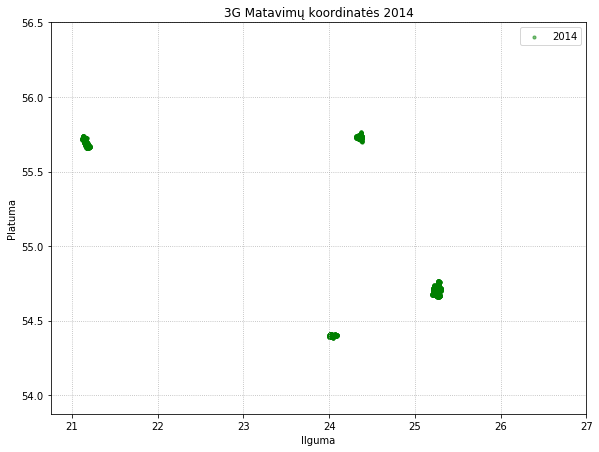
\includegraphics[scale=0.5]{img/3G-1}
	\caption{3G Matavimai 2014 metais. Viso – 2245 matavimai}
	\label{img:3G-1}
\end{figure}
\begin{figure}[H]
	\centering
	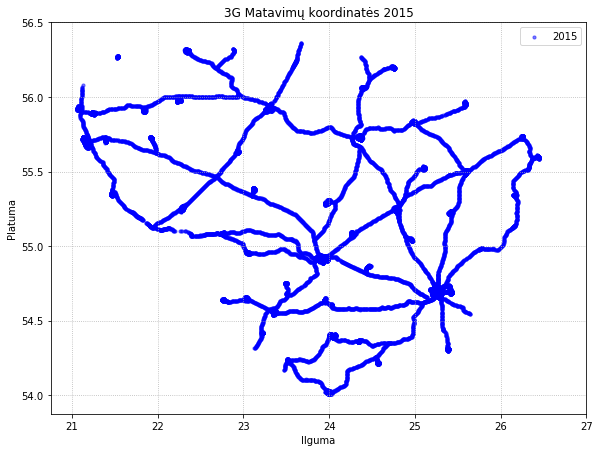
\includegraphics[scale=0.5]{img/3G-2}
	\caption{3G Matavimai 2015 metais. Viso – 19427 matavimai}
	\label{img:3G-2}
\end{figure}
\begin{figure}[H]
	\centering
	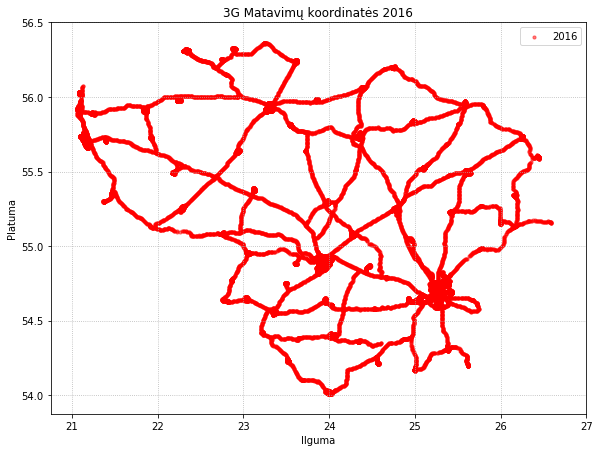
\includegraphics[scale=0.5]{img/3G-3}
	\caption{3G Matavimai 2016 metais. Viso – 34769 matavimai}
	\label{img:3G-3}
\end{figure}
\begin{figure}[H]
	\centering
	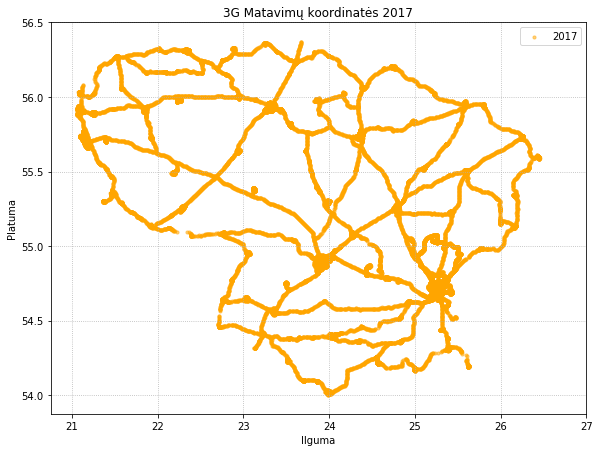
\includegraphics[scale=0.5]{img/3G-4}
	\caption{3G Matavimai 2017 metais. Viso – 38789 matavimai}
	\label{img:3G-4}
\end{figure}
\begin{figure}[H]
	\centering
	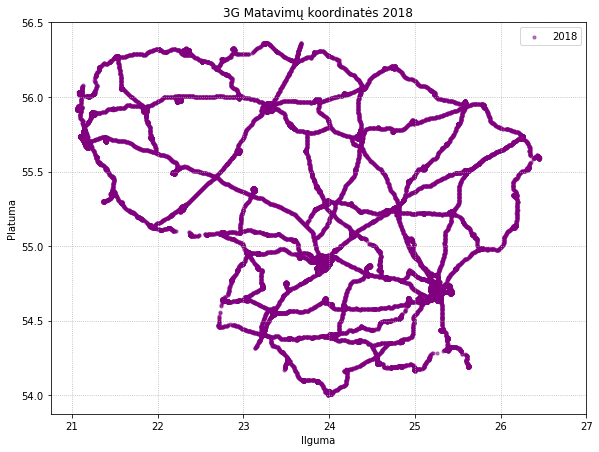
\includegraphics[scale=0.5]{img/3G-5}
	\caption{3G Matavimai 2018 metais. Viso – 40773 matavimai}
	\label{img:3G-5}
\end{figure}
IPSS \textbf{LTE} ryšio technologijos matavimai 2014–2018 metais. Viso 157522 įrašai.
\begin{figure}[H]
	\centering
	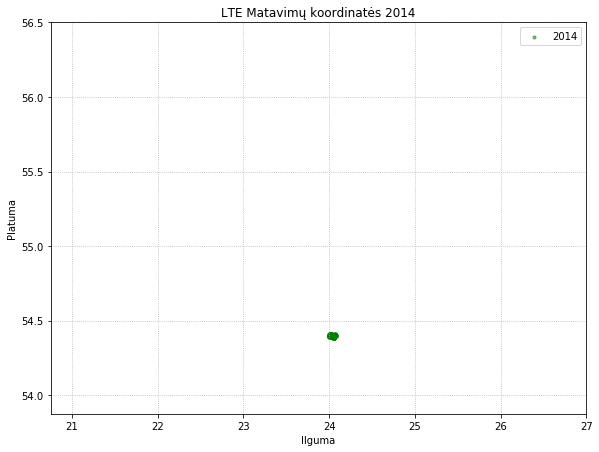
\includegraphics[scale=0.5]{img/LTE-1}
	\caption{LTE Matavimai 2014 metais. Viso – 232 matavimai}
	\label{img:LTE-1}
\end{figure}
\begin{figure}[H]
	\centering
	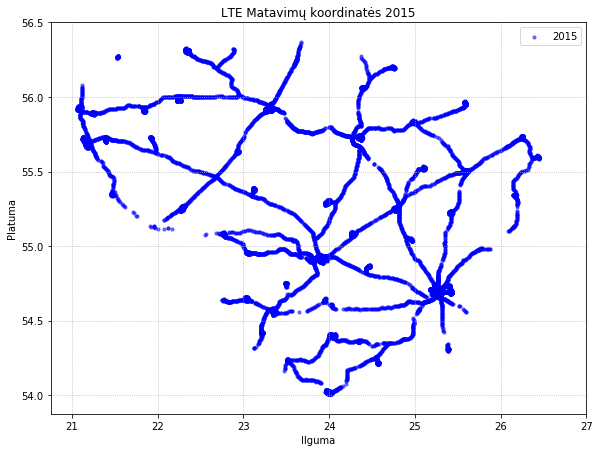
\includegraphics[scale=0.5]{img/LTE-2}
	\caption{LTE Matavimai 2015 metais. Viso – 13962 matavimai}
	\label{img:LTE-2}
\end{figure}
\begin{figure}[H]
	\centering
	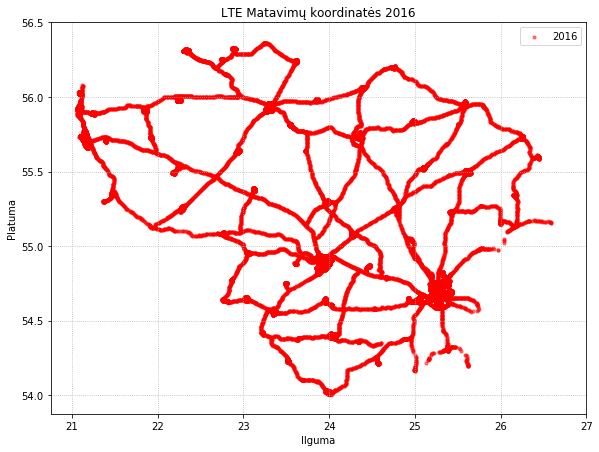
\includegraphics[scale=0.5]{img/LTE-3}
	\caption{LTE Matavimai 2016 metais. Viso – 40738 matavimai}
	\label{img:LTE-3}
\end{figure}
\begin{figure}[H]
	\centering
	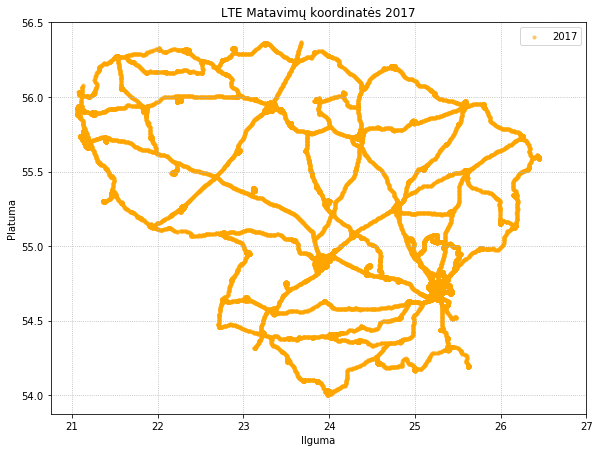
\includegraphics[scale=0.5]{img/LTE-4}
	\caption{LTE Matavimai 2017 metais. Viso – 49672 matavimai}
	\label{img:LTE-4}
\end{figure}
\begin{figure}[H]
	\centering
	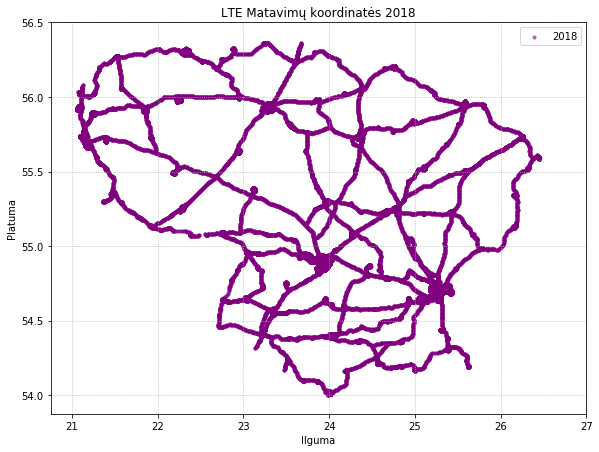
\includegraphics[scale=0.5]{img/LTE-5}
	\caption{LTE Matavimai 2018 metais. Viso – 52918 matavimai}
	\label{img:LTE-5}
\end{figure}
IPSS \textbf{WiMAX} ryšio technologijos matavimai 2014–2018 metais. Viso 18166 įrašai.
\begin{figure}[H]
	\centering
	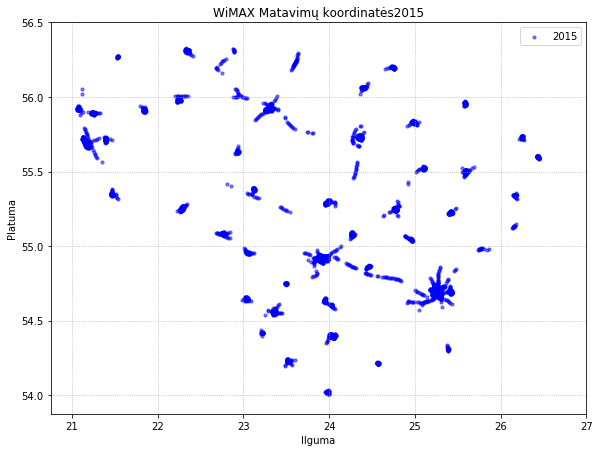
\includegraphics[scale=0.5]{img/WiMAX-1}
	\caption{WiMAX Matavimai 2015 metais. Viso – 4307 matavimai}
	\label{img:WiMAX-1}
\end{figure}
\begin{figure}[H]
	\centering
	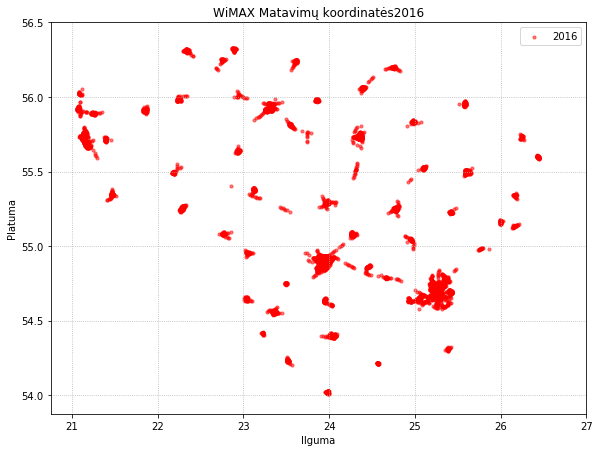
\includegraphics[scale=0.5]{img/WiMAX-2}
	\caption{WiMAX Matavimai 2016 metais. Viso – 7653 matavimai}
	\label{img:WiMAX-2}
\end{figure}
\begin{figure}[H]
	\centering
	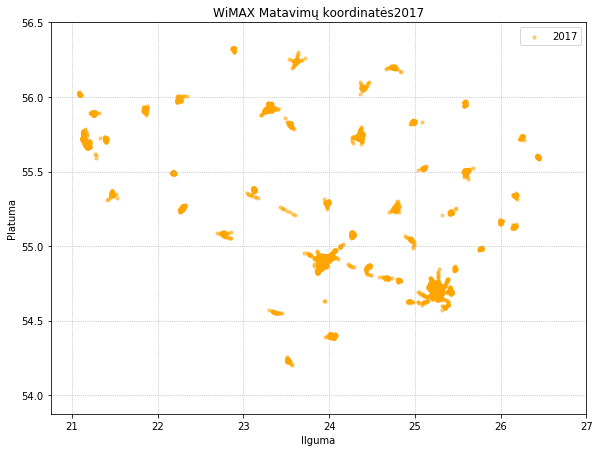
\includegraphics[scale=0.5]{img/WiMAX-3}
	\caption{WiMAX Matavimai 2017 metais. Viso – 6206 matavimai}
	\label{img:WiMAX-3}
\end{figure}

\section{Pradinių IPSS CSV failų apdorojimo „Python“ skriptas} \label{script1}
„Python“ skriptas „RenameAndRemoveFields.py“ skirtas iš duotųjų IPSS duomenų CSV failų atrinkti nereikalingus laukus ir pervadinti lietuviškus antraštės pavadinimus į vieno žodžio (vienos simbolių eilutės) angliškus pavadinimus bei sugeneruoti naujus CSV failus:
\lstinputlisting[language=Python]{scripts/RenameAndRemoveFields.py}

\section{Atrinktų IPSS CSV failų duomenų papildymo aukščio virš jūros lygio ir suapvalintų reikšmių laukais „Python“ skriptas} \label{script2}
„Python“ skriptas skirtas jau atrinktiems CSV failams pridėti papildomus laukus: aukščio virš jūros lygio (gaunamas iš koordinačių), suapvalintų koordinačių reikšmių bei suapvalintos aukščio reikšmės. Šiems duomenims yra sugeneruojamas nauji CSV failai:
\lstinputlisting[language=Python]{scripts/AddAltitudeAndRoundedColumns.py}

\section{Atrinktų IPSS CSV failų duomenų papildymo metų ir valandu laukais „Python“ skriptas} \label{script3}
„Python“ skriptas skirtas jau atrinktiems CSV failams pridėti papildomus laukus: metų ir valandų (gaunamas iš datos ir laiko). Šiems duomenims yra sugeneruojamas nauji CSV failai:
\lstinputlisting[language=Python]{scripts/AddYearAndHour.py}

\section{Atrinktų IPSS papildomų CSV failų generavimo „Python“ skriptas} \label{script4}
„Python“ skriptas skirtas jau atrinktiems CSV failams sugeneruoti skirtingų koordinačių ir aukščio virš jūros lygio reikšmių apvalinimo duomenų rinkinius. Šiems duomenims yra sugeneruojamas nauji CSV failai:
\lstinputlisting[language=Python]{scripts/GenerateMoreRoundedOptions.py}

\section{„MacroBase SQL“ SQL užklausų pavyzdys} \label{script4}
Darbo metu naudotos „MacroBase SQL“ SQL užklausos pavyzdys su pradiniais duomenimis, papildytais su aukščio virš jūros lygio ir suapvalintomis reikšmėmis duomenimis, ir papildytais metų bei valandų laukais duomenimis:
\lstinputlisting[language=Sql]{scripts/3G.sql}



\end{document}
